%!TEX root = ../Main.tex

\begin{figure}
\begin{center}
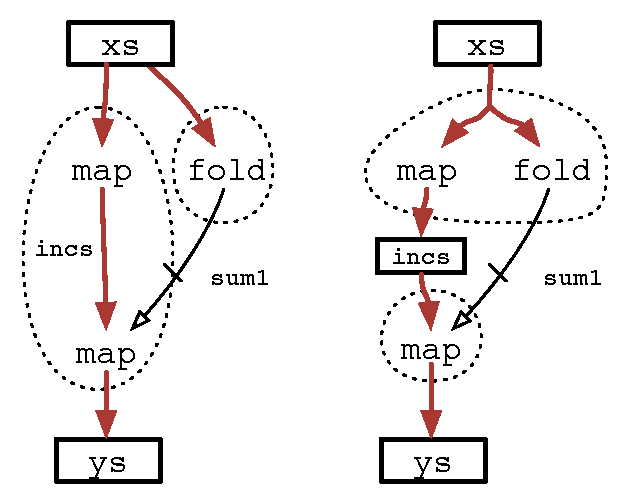
\includegraphics[scale=0.5]{figures/ex2-normalizeInc.pdf}
\end{center}
\caption{Possible clusterings for \texttt{normalizeInc}}
\label{f:normalizeInc}
\end{figure}


% -----------------------------------------------------------------------------
\section{Integer Linear Programming}
\label{s:ILP}
It is usually possible to cluster a program graph in multiple ways. For example, consider the following simple function:
\begin{code}
 normalizeInc :: Array Int -> Array Int
 normalizeInc xs
  = let incs = map  (+1)    us
        sum1 = fold (+) 0   us
        ys   = map  (/ sum) incs
    in  ys
\end{code}

Two possible clusterings are shown in Figure~\ref{f:normalizeInc}. One option is to compute @sum1@ first and fuse the computation of @incs@ and @ys@. Another option is to fuse the computation of @incs@ and @sum1@ into a single loop, then compute @ys@ separately. A third option (not shown) is to compute all results separately, and not perform any fusion. 

Which option is better? On current hardware we generally expect the cost of memory access to dominate runtime. The first clustering in Figure~\ref{f:normalizeInc} requires two reads from array @xs@ and one write to array @ys@. The second requires a single fused read from @xs@, one write to @incs@, a read back from @incs@ and a final write to @ys@. From the size constraints of the program we know that all intermediate arrays have the same size, so we expect the first clustering will peform better as it only needs three array accesses instead of four. 

For small programs such as @normalizeInc@ it is possible to naively enumerate all possible clusterings, select just those that are \emph{valid} with respect to fusion preventing edges, and chose the one that maximises a cost metric such as the number of array accesses needed. However, as the program size increases the number of possible clusterings becomes too large to naively enumerate. For example, Pouchet et al~\cite{pouchet2010combined} present a fusion system using the polyhedral model~\cite{pouchet2011polyhedral} and report that some simple numeric programs have over 40,000 possible clusterings, with one particular example having $10^{12}$. 

To deal with the combinatorial explosion in the number of potential clusterings, we instead use an Integer Linear Programming (ILP) formulation. ILP problems are defined as a set of variables, an objective linear function and a set of linear constraints. The integer linear solver finds an assignment to the variables that minimises the objective function, while satisfying all constraints. For the clustering problem we express our constraints regarding fusion preventing edges as linear constraints on the ILP variables, then use the objective function to encode our cost metric. This general approach was first fully described by Megiddo and Sarkar~\cite{megiddo1998optimal}, and our main contribution is to extend it to work with size changing operators such as @filter@. 



% -----------------------------------------------------------------------------
\subsection{Dependency Graphs}
A dependency graph represents the data dependencies of the program to be fused, and we use it as an intermediate stage when producing linear constraints for the ILP problem. The dependency graph contains enough information to determine the possible clusterings of the input program, while abstracting away from the exact operators used to compute each intermediate array. The rules for producing a dependency graphs are in Figure~\ref{f:DependencyGraph}.

Each binding in the source program becomes a node in the dependency graph. For each intermediate variable, we add a directed edge from the binding that produces a value to all bindings that consume it. Each edge is also marked as either \emph{fusible} or \emph{fusion preventing}. Fusion preventing edges are used when the producer must finish its execution before the consumer node can start. For example, a @fold@ operation must complete execution before it can produce the scalar value needed by its consumers. Conversely, the @map@ operation produces an output value for each value it consumes, so is marked as fusible. 

The @gather@ operation is a hybrid: it takes an indices array and an elements array, and for each element in the indices array returns the corresponding data element. This means that gather can be fused with the operation that produces its indices, but not the operation that produces its elements --- because those are accessed in a random-access manner. 

% Each node may simply be the name of its output binding (or bindings, in the case of @external@); as we require names to only be bound once, this is assured to be unique. Creating edges between these nodes is simply when one binding references an earlier one. The only complication is designating edges as \emph{fusible} or \emph{fusion-preventing}.

\begin{figure}
\begin{tabbing}
MMMMM       \= M  \= \kill
$nodes$     \> @:@ \> $\function \to V$              \\
$edges$     \> @:@ \> $\function \to E$              \\
$edge$      \> @:@ \> $\{bind\} \times bind \to E$ 
\\[1ex]
$nodes(bs)$ \> $= \{(name(b), \iiter_{\Gamma,C}(b)) | b \in bs\}$       
\\[2ex]

$edges(bs)$ \> $= \bigcup_{b \in bs}edge(bs, b)$    
\\[1ex]
MM             \= M \= \kill
$edge(bs, out = @fold@~f~in)$ \\
    \> $=$    \> $\{inedge(bs,out,s) | s \in fv(f)\} \cup \{inedge(bs, out, in) \}$       \\
$edge(bs, out = @map@~f~in)$  \\
    \> $=$    \> $\{inedge(bs,out,s) | s \in fv(f)\} \cup \{inedge(bs, out, in) \}$       \\
$edge(bs, out = @filter@~f~in)$  \\
    \> $=$    \> $\{inedge(bs,out,s) | s \in fv(f)\} \cup \{inedge(bs, out, in) \}$       \\
$edge(bs, out = @gather@~data~indices)$  \\
    \> $=$    \> $\{(out,data, \fusionpreventing) \} \cup \{inedge(bs, out, indices) \}$       \\
$edge(bs, out = @cross@~a~b)$            \\
    \> $=$    \> $\{inedge(bs, out, a) \}           \cup      \{(out, b, \fusionpreventing) \}$ \\
$edge(bs, outs = @external@~ins)$  \\
    \> $=$    \> $\{(outs,i, \fusionpreventing) | i \in ins \}$ 
\\[1ex]
$inedge(bs,to,\from)$ \\
    \> $|$ \> $(\from = @fold@~f~s) \in bs$     \\
    \> $=$ \> $(to, \from, \fusionpreventing)$  \\
    \> $|$ \> $(outs = @external@ \ldots) \in bs     \wedge \from \in outs$     \\
    \> $=$ \> $(to, outs, \fusionpreventing)$  \\
    \> $|$ \> $otherwise$                      \\
    \> $=$ \> $(to, \from, \fusible)$
\end{tabbing}

\caption{Dependency Graphs from Programs}
\label{f:DependencyGraph}
\end{figure}


\eject
% -----------------------------------------------------------------------------
\subsection{ILP Variables}
After generating the dependency graph, the next step is to produce a set of linear constraints from this graph. The variables involved in these constraints are split into three groups:
\begin{tabbing}
M   \= MM \= MMMMMMM \= MM \= \kill
$x$   \> @:@  \> $node \times node$ \> $\to$ \> $\mathbb{B}$
\end{tabbing}
For each pair of nodes with indices $i$ and $j$ we use a boolean variable $x_{ij}$ which indicates whether those two nodes are fused. We use $x_{ij} = 0$ when the nodes are fused and $x_{ij} = 1$ when they are not. Using $0$ for the fused case means that the objective function can be a weighted function of the $x_{ij}$ variables, and minimizing it tends to increase the number of nodes that are fused. The values of these variables are used to construct the final clustering, such that $\forall i,j.\ x_{ij} = 0 \iff cluster(i) = cluster(j)$.
\begin{tabbing}
M   \= MM \= MMMMMMM \= MM \= \kill
$\pi$ \> @:@  \> $node$             \> $\to$ \> $\mathbb{R}$
\end{tabbing}
The second group of variables is used to ensure that the clustering is acyclic. This means that for each node in the graph, the dependencies of that node can be executed before the node itself. For each node $i$, we associate a real $\pi_i$ such that every node $j$ that depends on $i$ we have $\pi_j > \pi_i$. Our linear constraints will ensure that if two nodes are fused into the same cluster then their $\pi$ values will be identical --- though nodes in different clusters can also have the same $\pi$ value.

Here is an example of a cyclic clustering:
\begin{code}
  cycle xs  = let ys  = map (+1) xs     (C1)
                  sum = fold ys         (C2)
                  zs  = map (+sum) ys   (C1)
              in  zs
\end{code}
There is no fusion-preventing edge directly between the @xs@ and @zs@ bindings, but there is a fusion-preventing edge between @sum@ and @zs@. If the @xs@ and @zs@ bindings were in the same cluster @C1@ and @sum@ was in cluster @C2@, there would be a dependency cycle between @C1@ and @C2@, and neither could be executed before the other.
\begin{tabbing}
M   \= MM \= MMMMMMM \= MM \= \kill
$c$   \> @:@  \> $node$             \> $\to$ \> $\mathbb{B}$
\end{tabbing}
The final group of variables is used to help define the cost model encoded by the objective function. Each node is assigned a variable $c_i$ that indicates whether the array the associated binding produces is \emph{fully contracted}. When an array is fully contracted it means that all consumers of that array are fused into the same cluster, so we have $c_i = 0 \iff \forall (i',j) \in E.\ i = i' \implies x_{ij} = 0$. In the final program, each successive element of a fully contracted array can be stored in a scalar register, rather than requiring an array register or memory storage. 


% -----------------------------------------------------------------------------
\subsection{Linear Constraints}
The constraints we place on the ILP variables are split into four groups: constraints that ensure the clustering is acyclic; constraints that encode fusion preventing edges; constraints on nodes with different iteration sizes, and constraints involving array contraction. 

% Before showing the optimised version with certain constraints removed (\S\ref{s:OptimisedConstraints}), this simpler, unoptimised version is shown. The only difference is that fewer constraints and variables are required in the optimised version, but both versions give the same clustering. This unoptimised version generates clustering constraints and variables for every pair of nodes, regardless of whether they may, in fact, be fused together. Later, we show that certain constraints and variables can be removed when there is a fusion-preventing edge between two nodes.


% -------------------------------------
\paragraph{Acyclic and precedence-preserving} The first group of constraints ensures that the clustering is acyclic:
\begin{tabbing}
MM  \= MMMx \= M \= MMM \= M \= MMMM \= \kill
    \> ~~~~~~~ $x_{i,j}$ \> $\le$ \> $\pi_j - \pi_i$ \> $\le$ \> $N.\; x_{i,j}$ 
    \>             (with an edge from $i$ to $j$)            \\
    \> $-N.\;  x_{i,j}$  \> $\le$ \> $\pi_j - \pi_i$ \> $\le$ \> $N.\; x_{i,j}$ 
    \>             (with no edge from $i$ to $j$)
\end{tabbing}
As per Megiddo~\cite{megiddo1998optimal} the form of these constraints is determined by whether there is an dependency between nodes $i$ and $j$. The $N$ value is set to the total number of nodes in the graph.

If there is an edge from node $i$ to $j$ we use the first constraint form shown above. If the two nodes are fused into the same cluster then we have $x_{i,j} = 0$. In this case the constraint simplifies to $0 \le \pi_j - \pi_i \le 0$, which forces $\pi_i = \pi_j$. If the two nodes are in \emph{different} clusters then the constraint instead simplifies to $1 \le \pi_j - \pi_i \le N$. This means that the difference between the two $\pi$s must be at least 1, and less than $N$. Since there are $N$ nodes, the maximum difference between any two $\pi$s would be at most $N$, so the upper bound of $N$ is large enough to be safely ignored. This means the constraint can roughly be translated to $\pi_i < \pi_j$, which enforces the acyclicity constraint.

If instead there is no edge from node $i$ to $j$ then we use the second constraint form above. As before, if the two nodes are fused into the same cluster then we have $x_{i,j} = 0$, which forces $\pi_i = \pi_j$. If the nodes are in different clusters then the constraint simplifies to $-N \le \pi_j - \pi_i \le N$, which effectively puts no constraint on the $\pi$ values.


% -------------------------------------
\paragraph{Fusion-preventing edges} As per Megiddo~\cite{megiddo1998optimal}, if there is a fusion preventing edge between two nodes we add a constraint to ensure the nodes will be placed in different clusters.
\begin{tabbing}
MMM     \= MMM \= M  \= MMM \= M \= MMM \= \kill
        \> $x_{i,j}$ \> $=$ \> $1$ \>   \> \\
        \> (for fusion-preventing edges from $i$ to $j$) 
\end{tabbing}
When combined with the precedence-preserving constraints earlier, setting $x_{i,j} = 1$ also forces $\pi_i < \pi_j$. 


% -------------------------------------
\paragraph{Fusion between different iteration sizes} This group of constraints restricts which nodes can be placed in the same cluster based on their iteration size. The group has three parts. 
Firstly, either of the two nodes connected by an edge have an unknown ($\bot$) iteration size then they cannot be fused and we set $x_{i,j} = 1$:
\begin{tabbing}
MMM     \= MMM \= M \= MMM \= M \= MMM \= \kill
        \> $x_{i,j}$   \> $=$   \> $1$          \>       \>     \\
        \> (if $\iiter_{\Gamma,C}(i) = \bot 
                ~\vee~ \iiter_{\Gamma,C}(j) = \bot$)
\end{tabbing}
Secondly, if the two nodes have different iteration sizes and no common parent then they also cannot be fused and we set $x_{i,j} = 1$:
\begin{tabbing}
MMM     \= MMM \= M \= MMM \= M \= MMM \= \kill
        \> $x_{i,j}$   \> $=$   \> $1$          \>       \>     \\
        \> (if $\iiter_{\Gamma,C}(i) \not= \iiter_{\Gamma,C}(j) 
                ~\wedge~ parents(i,j) = \emptyset$)
\end{tabbing}
Finally, if the two nodes had different iteration sizes but \emph{do} have parent transducers of the same size, then the two nodes can be fused if they are fused with their respective parents, and the parents themselves are fused:
\begin{tabbing}
MMM     \= MMM \= M \= MMM \= M \= MMM \= \kill
        \> $x_{a,A}$   \> $\le$ \> $x_{a,b}$    \>       \>     \\
        \> $x_{b,B}$   \> $\le$ \> $x_{a,b}$    \>       \>     \\
        \> $x_{A,B}$   \> $\le$ \> $x_{a,b}$    \>       \>     \\
        \> (if $\iiter_{\Gamma,C}(a) \not= \iiter_{\Gamma,C}(b) 
                ~\wedge~ parents(a,b) = \{(A,B)\}$)
\end{tabbing}
This last part is the main difference to existing ILP solutions: we allow nodes with different iteration sizes to be fused when their parent transducers are fused. The actual constraints encode a ``no more fused than'' relationship. For example $x_{a,A} \le x_{a,b}$ means that nodes $a$ and $b$ can be no more fused than nodes $a$ and $A$. 

As a simple example, consider fusing an operation on filtered data with its generating filter:
\begin{code}
    sum1 = fold (+) 0  xs
    gts  = filter (>0) xs
    sum2 = fold (+) 0  gts
\end{code}
Here $sum1$ and $sum2$ have different iteration sizes and we have that $parents(sum1, sum2) = \{(sum1, gts)\}$. This means that $sum1$ and $sum2$ may only be fused if $sum1$ is fused with $sum1$ (trivial), $sum2$ is fused with $gts$, and $sum1$ is fused with $gts$.

% Here, $parents(gts,sum2) = \{gts, gts\}$. This generates spurious, but still valid, constraints that $gts$ must be fused with $gts$ and $gts$ must be fused with $sum2$, in order for $gts$ and $sum2$ to be fused together. While these constraints are unnecessary in this case, they are harmless.

% While it may seem like these constraints should be implied by transitivity of clustering, all clustering variables are used for the objective function.


% -------------------------------------
\paragraph{Array contraction} The final group of constraints gives meaning to the $c$ variables that we use to represent whether an array is fully contracted:
\begin{tabbing}
MMM     \= MMM \= M \= MMM \= M \= MMM \= \kill
        \> $x_{ij}$    \> $\le$ \> $c_i$  \> \> \\
        \> (for all edges from i)
\end{tabbing}
Recall that an array is fully contracted when all of the consumers are fused with the nodes that produces it, which means that the array does not need to be fully materialized in memory. As per Darte's work on array contraction~\cite{darte2002contraction}, we define a variable $c_i$ for each array, and the constraint above ensures that $c_i = 0$ only if $\forall (i',j) \in E.\ i = i' \implies x_{ij} = 0$. By minimizing $c_i$ in the objective function, we favor solutions that reduce the number of intermediate arrays.


% -----------------------------------------------------------------------------
\subsection{The Objective Function}
\label{s:ObjectiveFunction}

To find the objective function, note that fusing loops can have three main benefits:
\begin{itemize}
\item
reducing memory traffic, such as multiple loops reading from the same array;
\item
removing intermediate arrays, thus reducing the amount of memory required;
\item
and reducing loop overhead, such as when two loops operate on different arrays of the same size.
\end{itemize}
However, these benefits cannot be considered in isolation; for example, fusing two loops to reduce loop overhead may remove potential fusion opportunities that reduce memory traffic.
When operating on large arrays that do not fit in cache, memory traffic dominates execution time.
An excessive number of intermediate arrays can also cause issues if all are live in memory at once, potentially leading to \emph{thrashing}.
The benefits of removing loop overhead are least of all; it should be performed if possible, but must never remove opportunities for other fusion. \TODO{Refer to example code that demonstrates these different opportunities.}

This total ordering can be encoded into an ILP objective function as weights.
If the program graph contains $N$ combinators, then there are at most $N$ opportunities for fusion.
The encoding of loop overhead is weight $1$, removing intermediate arrays is weight $N$, and reducing memory traffic is weight $N^2$.
This ensures that no amount of loop overhead reduction can outweigh the benefit of removing an intermediate array,
and likewise no number of removed intermediate arrays can outweigh a reduction in memory traffic.
Although, it is worth noting that reducing memory traffic does \emph{tend} to remove intermediate arrays, and vice versa.

\begin{tabbing}
MMMMM   \= MMMM \= M \= \kill
Minimise   \>     \> $\Sigma_{(i,j) \in E} W_{ij} x_{ij}$   \\
           \> \> \> (memory traffic and loop overhead)         \\
           \> $+$ \> $\Sigma_{i \in V} N c_i$  \\
           \> \> \> (removing intermediate arrays)         \\
Subject to \> \ldots                                \\
Where      \>                                       \\
           \> $W_{ij} = N^2$ \> $~|$ \> $(i,j) \in E $         \\
           \> \> \> (fusing $i$ and $j$ will reduce memory traffic)         \\
           \> $W_{ij} = N^2$ \> $~|$ \> $\exists k. (k,i) \in E \wedge (k,j) \in E $     \\
           \> \> \> ($i$ and $j$ share an input array)                                         \\
           \> $W_{ij} = 1$   \> $~|$ \> $@otherwise@$                                                  \\
           \> \> \> (the only benefit is loop overhead)                                        \\
           \\
           \> $N = |V|$
\end{tabbing}


% -----------------------------------------------------------------------------
\subsection{Transitivity of Clustering}
It may seem that we could generate far fewer constraints and rely on transitivity of clustering equality $x_{ij}$.
This means that for each pair $i,j$ we would only generate an $x_{ij}$ and constraints, if $i$ or $j$ is a @filter@, or there is an edge between $i$ and $j$.
This would simplify the integer linear program, but would also modify the objective function not to \emph{minimise} on these removed $x_{ij}$.
The objective function of this simplified version would not count the benefits of fusing two non-connected nodes, and would not reduce memory traffic as effectively.


% -----------------------------------------------------------------------------
\subsection{Fusion-preventing Path Optimisation}
\label{s:OptimisedConstraints}
We can remove certain constraints and variables, by only checking nodes if there is no \emph{fusion-preventing path} between $i$ and $j$.
If there is a fusion-preventing path between two nodes, they are known to be in different clusters.
With our specific knowledge of the problem domain, we can simplify the integer linear program and make the job of the ILP solver easier by omitting these constraints.
Creating fewer constraints and variables should make it faster for the ILP solver to find a solution.

For the graph, we define a function $split(a,b)$ to check whether there exists a fusion-preventing path between two nodes, $a$ and $b$.

\begin{tabbing}
MMM      \= MM   \=  MMMMMMMMMMMM    \=  \kill
$split$     \> @::@ \> $name \times name \to \mathbb{B}$      \\
MM        \= M    \= \kill
$split(a,b)$ \\
    \>$=$  \>$\forall p \in path(a,b) \cup path(b,a).\ \fusionpreventing \not\in p$\\
\end{tabbing}

With $split$ defined, we can refine our formulation to only generate constraints between two nodes if there is a chance they may be fused together.
The entire formulation of the integer linear program follows.

\begin{tabbing}
MMMMM   \= MMM \= M \= MMM \= M \= MMM \= \kill
Minimise   \> $\Sigma_{(i,j) \in E} W_{ij} x_{ij} + \Sigma_{i \in V} N c_i$  \\
           \> (if $split(i,j)$)         \\
Subject to \\
           \> $-N x_{ij}$ \> $\le$ \> $\pi_j - \pi_i$ \> $\le$ \> $N x_{ij}$ \\
           \> (if $split(i,j) \wedge (i,j) \not\in E \wedge (j,i) \not\in E$)            \\
\\
           \>    $x_{ij}$ \> $\le$ \> $\pi_j - \pi_i$ \> $\le$ \> $N x_{ij}$ \\
           \> (if $split(i,j) \wedge (i,j,\fusible) \in E$)     \\
\\
           \>             \>       \> $\pi_i < \pi_j$ \>       \>            \\
           \> (if $(i,j,\fusionpreventing) \in E$)    \\
\\
           \> $x_{ij}$    \> $\le$ \> $c_i$           \>       \>            \\
           \> (if $split(i,j)$) \\
           \> $c_{i }$    \> $ = $ \> $ 1 $           \>       \>            \\
           \> (if $\neg(split(i,j))$) \\
\\
           \> $x_{ij}$    \> $=$   \> $1$             \>       \>            \\
           \> (if $\iiter_{\Gamma,C}(i) \not= \iiter_{\Gamma,C}(j) \wedge parents(i,j) = \emptyset$)  \\
           \\
           \> $x_{ij}$    \> $=$   \> $1$             \>       \>            \\
           \> (if $\bot \in \{\iiter_{\Gamma,C}(i), \iiter_{\Gamma,C}(j)\}$)  \\
           \\
           \> $x_{i'j}$   \> $\le$ \> $x_{ij}$        \>       \>            \\
           \> $x_{ij'}$   \> $\le$ \> $x_{ij}$        \>       \>            \\
           \> $x_{i'j'}$   \> $\le$ \> $x_{ij}$        \>       \>            \\
           \> (if $\iiter_{\Gamma,C}(i) \not= \iiter_{\Gamma,C}(j) \wedge parents(i,j) = \{i',j'\} \wedge$ \\

           \> \> $ split(i,j) \wedge split(i',j) \wedge split(i,j') \wedge split(i',j') $) \\
MMMMM   \= MMMM \= M \= \kill
Where      \>                                       \\
           \> $W_{ij} = N^2$ \> $~|$ \> $(i,j) \in E $         \\
           \> \> \> (fusing $i$ and $j$ will reduce memory traffic)         \\
           \> $W_{ij} = N^2$ \> $~|$ \> $\exists k. (k,i) \in E \wedge (k,j) \in E $     \\
           \> \> \> ($i$ and $j$ share an input array)                                         \\
           \> $W_{ij} = 1$   \> $~|$ \> $@otherwise@$                                                  \\
           \> \> \> (the only benefit is loop overhead)                                        \\
           \\
           \> $N = |V|$
\end{tabbing}

% % !!!!!!!!!!!!!!!!!!!!!!!
% I commented the \input out in section/04-ILP.tex

\subsection{Proof}
To prove correctness of our linear program formulation, we need to prove two different things.
Firstly, the formulation's constraints must always be satisfiable; that is, there must exist a variable assignment that satisfies all constraints.
This is rather simple to show, but guarantees that the linear program will always give an answer.
The next thing to show is that any produced clustering is legal: if a variable assignment satisfies the constraints, then it is a valid and legal clustering.
This means that, not only do we get \emph{an} answer, we also get the \emph{right} answer.

%!TEX root = ../Main.tex
\subsubsection{Satisfiability}
For any program $p$, there exists a trivial clustering with no fusion at all.
We can use this as the variable assignment of $ilp(p)$.
For each pair of nodes $m,n \in p$, $x_{mn} = 1$ --- no fusion is possible.
For the $\pi$ variables, we must find a topographical ordering of the nodes in $p$, which is simple since we are assured it is a dag.

\TODO{Now, prove that this assignment actually satisfies the constraints.}


\subsubsection{Soundness}
For any program $p$ and variable asignment $v$, if $v$ satisfies the constraints for $ilp(p)$, the clustering denoted by $x_{ij}$ in $v$ is legal.

For a clustering to be legal, it must satisfy three constraints:
\begin{description}
\item[Acyclic]
after merging nodes of same cluster together, the resulting graph must be a dag
\item[Precedence preserving]
if there is an edge between two nodes $i$ and $j$, and they are not merged together, then we require $\pi_j > \pi_i$
\item[Fusion preventing]
likewise, if there is a fusion-preventing edge between two nodes $i$ and $j$, then we require $\pi_j > \pi_i$, which implies that they are not merged together
\item[Type constraint]
if two nodes $i$ and $j$ are in the same cluster, then $\tau_i = \tau_j$, or if $\tau_i$ is a subtype of $\tau_j$ (or $\tau_j$ is a subtype of $\tau_i$), then the \emph{generator} for $\tau_i$ (or $\tau_j$) must also be in the same cluster as $i$ and $j$.
    \\
    \TODO Actually, let us say $x_{ij} = 0 \implies check_{ij}$

\end{description}
where
\begin{tabbing}
MMMMM      \= M \= MMMMMMM \= MM \= \kill
$check$ \> @::@  \> $array \times array$ \> $\to$ \> $\mathbb{B}$ \\
MMMMM      \= M \= MMMMMM \= MM \= \kill
$check(i, j)$     \> $|$ \> $tau_i = tau_j$ \> $=$ \> $x_{i,j} = 0$                        \\
$check(i, j)$     \> $|$ \> $i' \in gen(i) $ \> $=$ \> $x_{i',j} = 0 \wedge x_{i,i'} = 0 \wedge check(i', j)$                        \\
$check(i, j)$     \> $|$ \> $j' \in gen(j) $ \> $=$ \> $x_{i,j'} = 0 \wedge x_{j,j'} = 0 \wedge check(i, j')$                        \\
$check(i, j)$     \> $|$ \> $tau_i \not= tau_j$\> $=$ \> $\bot$
\end{tabbing}








